\section{Resultados}
%Deben incluir los resultados de los experimentos, utilizando el formato más adecuado
%para su presentación. Deberón especificar claramente a qué experiencia corresponde
%cada resultado. No se incluirán aquí corridas de máquina. Algo fundamental en su
%aprendizaje en la materia es la presentación de resultados de forma clara y concisa para
%el lector.

\subsection{Experimento 1}

\subsubsection{Primer caso}

Para el primer caso lo que se hizo fue trabajar con un parabrisas de tamaño PARxPAR (a par y b par). En el caso de la función dameTempPtoCritico ésta representacion entra como el caso IMPARxIMPAR (ya que recordemos que se resta una unidad a las medidas de ancho y alto para no contar los bordes). De esta forma, la temperatura en el punto crítico esta dada por un solo punto.
El radio de las sanguijuelas puede variar hasta los 15 metros, para tener una mayor diversidad de tamaños, y tratar de verificar lo planteado en la hipótesis5.\newline
Se trabajó con 3 discretizaciones distintas 2, 5 y 10. Los resultados se pueden observar en los gráficos: \textit{figure 1.a, figura 1.b y figure 1.c}

%140x140
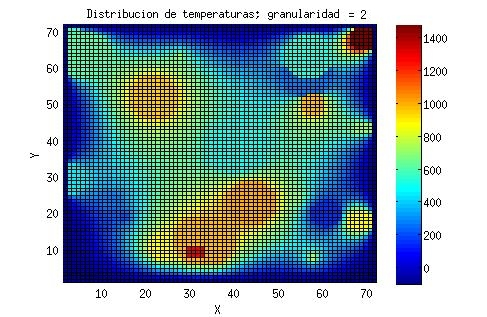
\includegraphics[width=\textwidth,height=3.0in,keepaspectratio
]{140x140h2.jpg} \newline
\begin {flushleft}
\textbf{Figure 1.a:} Distribución de temperaturas para un parabrisas con a = 140 metros; b = 140 metros; h = 2; n = 25. Donde el radio máximo de cada sanguijuela es 15 metros. Y la temperatura en el punto crítico es de 499.00000\hspace{-1.5mm}$\phantom{a}^{\circ}$c .
\end{flushleft}

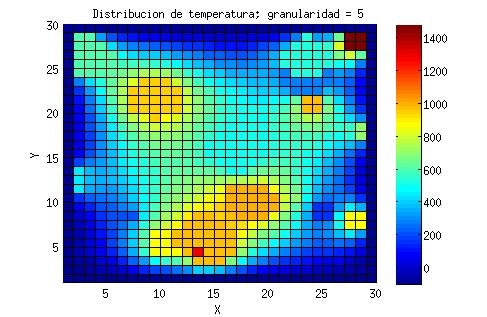
\includegraphics[width=\textwidth,height=3.0in,keepaspectratio
]{140x140h5.jpg} \newline
\begin {flushleft}
\textbf{Figure 1.b:} Mismas características que para el parabrisas representado en la $figure$ $1.a$. Pero, con granularidad igual a 5. La temperatura en el punto crítico es de 499.00000\hspace{-1.5mm}$\phantom{a}^{\circ}$c.
\end{flushleft}


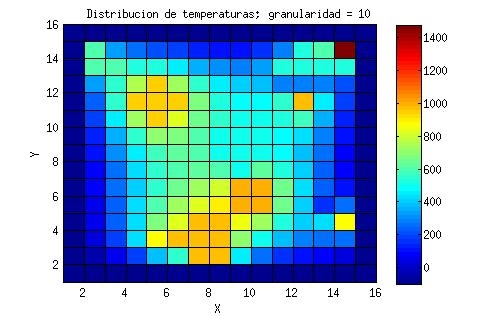
\includegraphics[width=\textwidth,height=3.0in,keepaspectratio
]{140x140h10.jpg} \newline
\begin {flushleft}
\textbf{Figure 1.c:} Mismas características que para el parabrisas representado en la $figure$ $1.a$. Pero, con granularidad igual a 10 y cuya temperatura en el punto crítico es de 499.00000\hspace{-1.5mm}$\phantom{a}^{\circ}$c .
\end{flushleft}


\subsubsection{Segundo caso}


%45x45

Otro caso que analizamos fue trabajar con un parabrisas de tamaño IMPARxIMPAR (lo que se corresponde al caso PARxPAR, al momento de obtener la temperatura en el punto crítico). El mótivo de trabajar con este caso, fue que como consecuencias de las dimensiones del parabrisas la temperatura en el punto crítico ahora depende de 4 valores en total. Basta con que al menos uno de los mismos se modifique, entre las distintas discretizaciones, para que la temperatura en el punto crítico cambie. Esta idea es la que se refleja en la hipótesis3.\newline
Ademas, se trabajó con una granularidad menor a uno en este caso. Ya que a diferencia de los restantes las dimensiones del parabrisas son menores y dado que al momento de discretizar. Los parametros ancho y alto son dividos por la granularidad, el sistema cuenta con mas puntos que para los valores mayores e iguales a 1. Y para parabrisas de mayor tamaño el tiempo de computo sería excesivamente caro.  
Una caracteristica de esta experimentación es que predominan las denominadas Sanguijuelas unitarias. Dicha elección se realizo para tratar de verificar la hipótesis4. Los resultados obtenidos son los presentados en los gráficos \textit{figure 2.a, figure 2.b, figure 2.c y figure 2.d}\newline


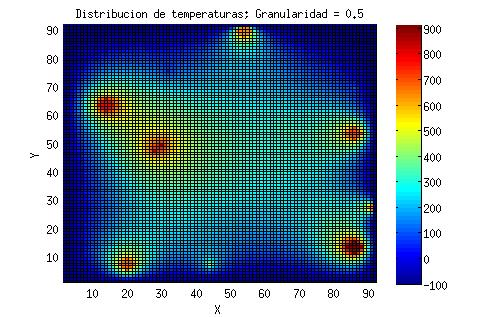
\includegraphics[width=\textwidth,height=3.0in,keepaspectratio
]{45x45h0,5.jpg} \newline
\begin {flushleft}
\textbf{Figure 2.a:} Distribución de temperaturas para un parabrisas con a = 45 metros; b = 45 metros; h = 0.5; n = 15. Donde el radio máximo de cada sanguijuela es de 2 metros. Y la temperatura en el punto crítico es de  350.69248\hspace{-1.5mm}$\phantom{a}^{\circ}$c .
\end{flushleft}

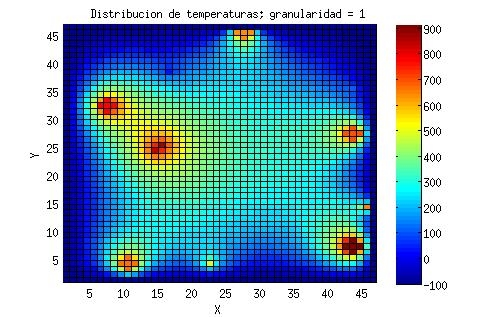
\includegraphics[width=\textwidth,height=3.0in,keepaspectratio
]{45x45h1.jpg} \newline
\begin {flushleft}
\textbf{Figure 2.b:} Mismas características que para el parabrisas representado en la $figure$ $2.a$. Pero, con granularidad igual a 5 y cuya temperatura en el punto crítico de 370.11472\hspace{-1.5mm}$\phantom{a}^{\circ}$c .
\end{flushleft}

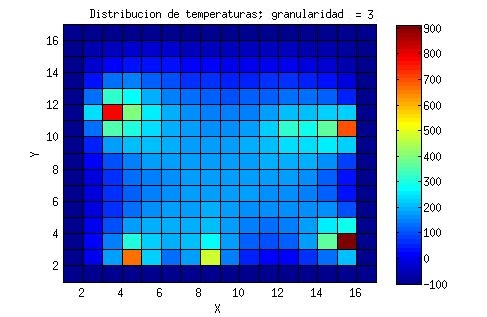
\includegraphics[width=\textwidth,height=3.0in,keepaspectratio
]{45x45h3.jpg} \newline
\begin {flushleft}
\textbf{Figure 2.c:} Se varía la granularidad del parabrisas representado por la $figure$ $2.a$ a 3. La temperatura en el punto crítico, de esta nueva representación, es de 175.58285\hspace{-1.5mm}$\phantom{a}^{\circ}$c .
\end{flushleft}

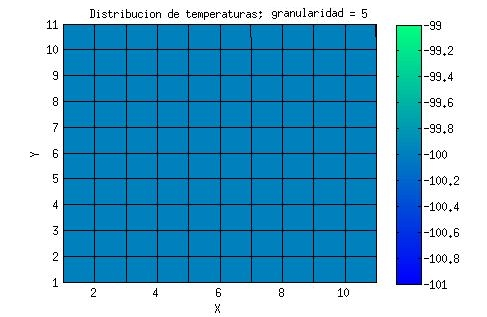
\includegraphics[width=\textwidth,height=3.0in,keepaspectratio
]{45x45h5.jpg} \newline
\begin {flushleft}
\textbf{Figure 2.d:} Mismas características que para el parabrisas representado en la $figure$ $2.a$. Pero, con granularidad igual a 5 y cuya temperatura en el punto crítico es de -100.00000\hspace{-1.5mm}$\phantom{a}^{\circ}$c.
\end{flushleft}


\subsubsection{Tercer caso}


Para continuar con la idea de ver cuanto difiere las temperaturas en un parabrisas de tamaño IMPARxIMPAR. Pero, sobre todo para corroborar la hipótesis4. Se trabajó con el mismo parabrisas que en el caso anterior. Porlo que ahora se aumentó el radio de acción de las sanguijuelas de manera que haya una mayor diversidad de sanguijuelas. Ademas, que de esta forma vamos a poder conluir como afecta el radio de una sanguijuela sobre un mismo sistema. Los datos obtenidos se muestran en las figuras: \textit{figure 3.a, figure 3.b, figure 3.c}  \newline


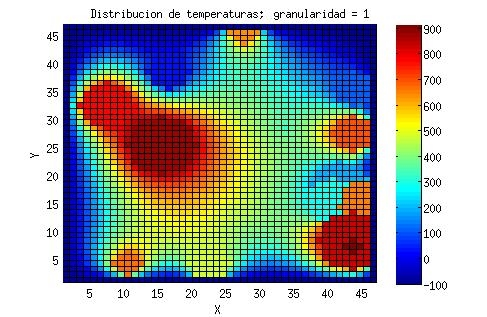
\includegraphics[width=\textwidth,height=3.0in,keepaspectratio
]{r7h1.jpg} \newline
\begin {flushleft}
\textbf{Figure 3.a:} Representación de la distribución de temperaturas para un parabrisas con a = 45 metros; b = 45 metros; h = 1; n = 15. Donde el radio máximo de cada sanguijuela es 8 metros. Y la temperatura alcanzada en el punto crítico es de 644.83827\hspace{-1.5mm}$\phantom{a}^{\circ}$c .
\end{flushleft}

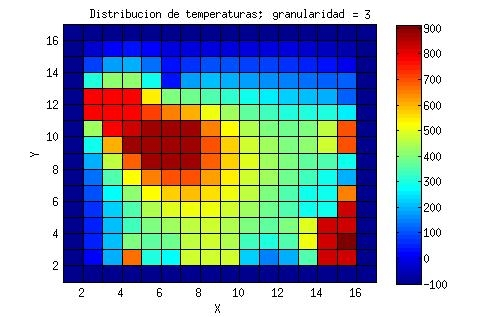
\includegraphics[width=\textwidth,height=3.0in,keepaspectratio
]{r7h3.jpg} \newline
\begin {flushleft}
\textbf{Figure 3.b:} Mismas características que para el parabrisas representado en la $figure$ $3.a$. Pero, con granularidad igual a 3. Y la temperatura alcanzada en el punto crítico es de 633.08219\hspace{-1.5mm}$\phantom{a}^{\circ}$c .
\end{flushleft}

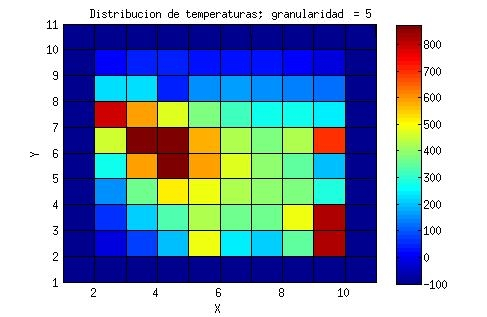
\includegraphics[width=\textwidth,height=3.0in,keepaspectratio
]{r7h5.jpg} \newline
\begin {flushleft}
\textbf{Figure 3.c:} Mismas características que para el parabrisas representado en la $figure$ $3.a$. Pero, con granularidad igual a 5 y cuya temperatura en el punto crítico es igual a 515.79566\hspace{-1.5mm}$\phantom{a}^{\circ}$c .
\end{flushleft}


\subsubsection{Cuarto caso}


Debido a que en los anteriores caso el valor del punto crítico dependia de uno o cuatro valores. Se decidió ver la última variante que existe, que es cuando un parabrisas tiene un lado par y el otro impar. De esta forma, el punto crítico depende del promedio entre dos valores. \newline
Este caso nos resulta útil para tratar de corroborar la veracidad de la hipótesis3. Para acercanos a un caso promedio en el que no solo van a aparecer sanguijuelas con radio acción bajo, el mismo puede variar hasta los 10 metros. Los gráficos presentados a continuación reflejan los datos obtenidos.    

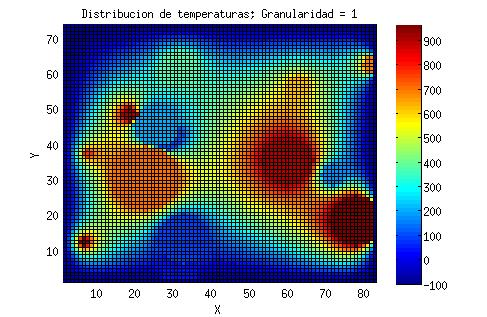
\includegraphics[width=\textwidth,height=3.0in,keepaspectratio
]{82x71h1.jpg} \newline
\begin {flushleft}
\textbf{Figure 4.a:} Representación de la distribución de temperaturas para un parabrisas con a = 81 metros; b = 71 metros; h = 1; n = 15. Donde el radio máximo de cada sanguijuela es de 10 metros. La temperatura en el punto crítico es de 533.86579\hspace{-1.5mm}$\phantom{a}^{\circ}$c .
\end{flushleft}

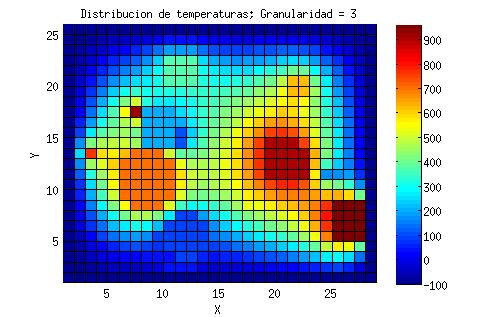
\includegraphics[width=\textwidth,height=3.0in,keepaspectratio
]{82x71h3.jpg} \newline
\begin {flushleft}
\textbf{Figure 4.b:} Mismas características que para el parabrisas representado en la $figure$ $4.a$. Pero, con granularidad igual a 3. Y la temperatura alcanzada en el punto crítico es de 495.18948\hspace{-1.5mm}$\phantom{a}^{\circ}$c .
\end{flushleft}

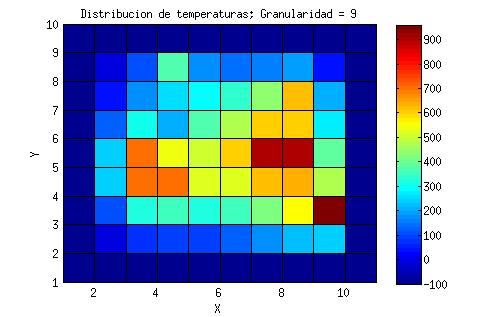
\includegraphics[width=\textwidth,height=3.0in,keepaspectratio
]{82x71h9.jpg} \newline
\begin {flushleft}
\textbf{Figure 4.c:} Mismas características que para el parabrisas representado en la $figure$ $4.a$. Pero, con granularidad igual a 5 y cuya temperatura en el punto crítico es de 552.85704\hspace{-1.5mm}$\phantom{a}^{\circ}$c .
\end{flushleft}








\subsection{Experimento 2}
\subsubsection{Experimento relación tiempo-calidad de cómputo}
Las siguientes tres tablas representan los datos tomados de tres instancias del problema. Lo único que vamos a variar en dichas instancias son los radios de las sanguijuelas. Para las tres instancias $a = 20$, $b = 20$, la cantidad de sanguijuelas es 8 y las ubicaciones y temperaturas (variando en un rango de 50 a 730) de cada sanguijuela son las mismas (pueden encontrarse en los archivos de Experimentos/Experimento2/instancias20x20).
\newline
\begin{figure}[H]
\centering
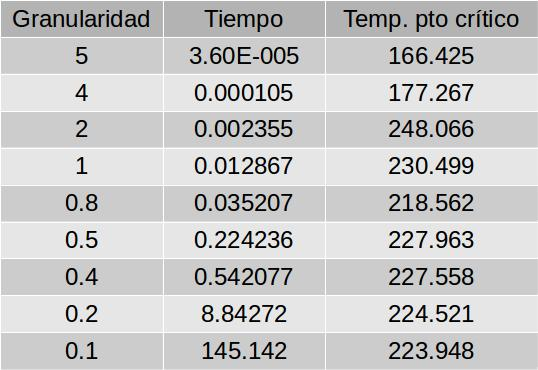
\includegraphics[scale=0.4]{instancia20x20_1.jpg}\caption{En este conjunto de instancias los radios de las sanguijuelas están en el conjunto $\{2, 3, 4\}$. Podemos observar como efectivamente el tiempo crece cuando el parámetro $h$ de granularidad disminuye. En cuanto a la temperatura del punto crítico, se puede ver como a medida que aumentamos el tamaño de nuestras discretizaciones, se va acercando a un valor cercano a 224 grados.}
\end{figure}

\begin{figure}[H]
\centering
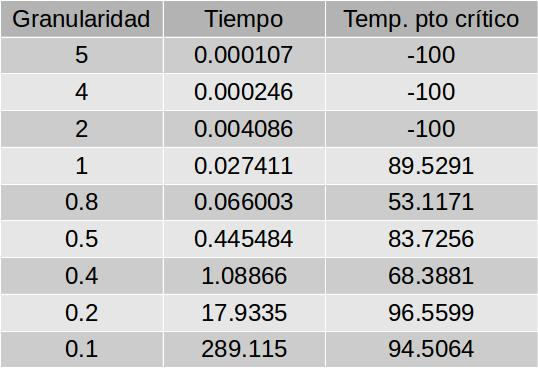
\includegraphics[scale=0.4]{instancia20x20_2.jpg}\caption{En este otro experimento, hemos decidido achicar considerablemente los radios de las sanguijuelas de manera que estén en el rango $[0.03, 1]$. Por un lado, podemos ver que el tiempo sigue aumentando a medida que $h$ disminuye al igual que en el experimento anterior. Sin embargo, se puede ver también que el algoritmo toma más tiempo que antes en resolver cada instancia. De todas formas, lo más llamativo parece encontrarse en las primeras tres entradas de la tabla, en los valores de temperatura del punto crítico. Pareciera como si las primeras tres discretizaciones de nuestro modelo del problema, aproximan tan mal al caso real que quedan descartadas todas las sanguijuelas. Sin embargo, al igual que en el experimento anterior, se cumple que a medida que aumenta el tamaño de la discretización, la temperatura en el punto crítico se acerca a un valor.}
\end{figure}

\begin{figure}[H]
\centering
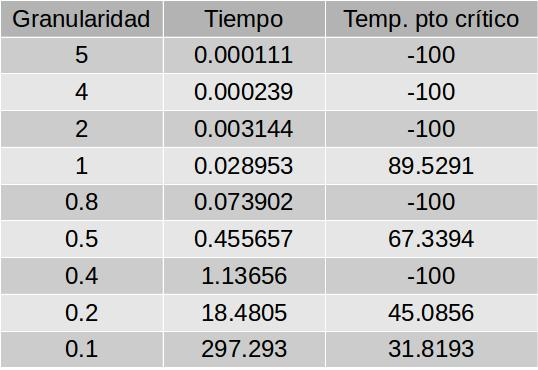
\includegraphics[scale=0.4]{instancia20x20_3.jpg}\caption{Una vez más, volvemos a achicar los radios de las sanguijuelas. Vemos que el tiempo se sigue comportando de manera similar y con las primeras tres instancias del problema ocurre lo mismo que con el experimento anterior. Sin embargo, ahora si está sucediendo algo que contradice una de las hipótesis (la tercera) planteada en el desarrollo ya que vemos que ahora, no pareciera que nos estemos acercando a un valor (el valor de la solución real). Esto se ve en las entradas 6 y 7 de la tabla, cuyas granularidades son 0.8 y 0.4, donde a pesar de que son más chicas que 1 (y por lo tanto las discretizaciones poseen tamaños más grandes), se está obteniendo -100 como temperatura del punto crítico, lo cuál no parece estar bien.}
\end{figure}

\begin{figure}[H]
\centering
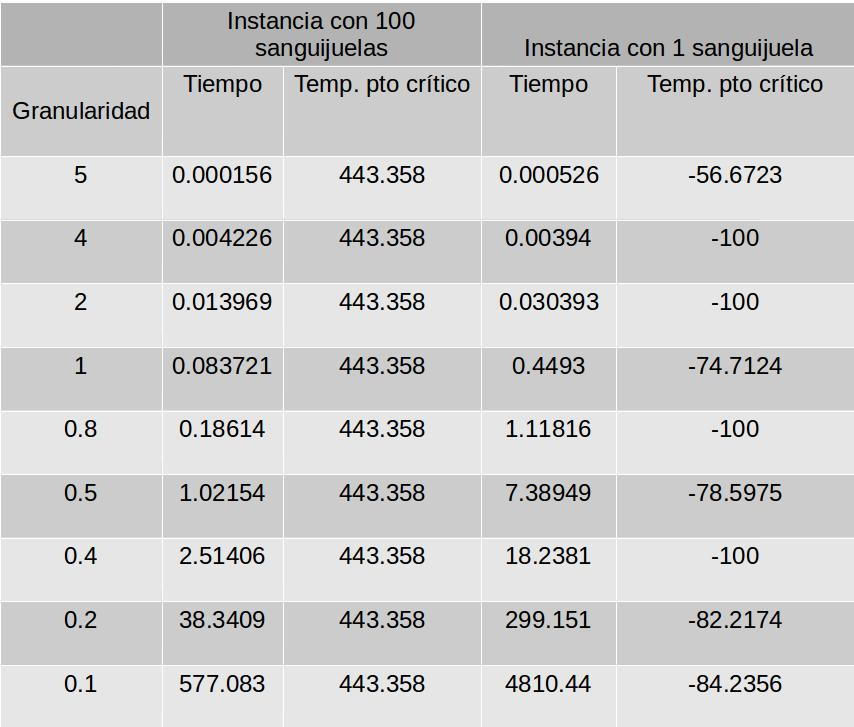
\includegraphics[scale=0.4]{instancias40x40.jpg}\caption{En este experimento se trabajó con dos instancias, esta vez ambas de 40x40 y con distintas sanguijuelas asociadas a una y a otra. Más específicamente y como indica la tabla, en una instancia hay 100 sanguijuelas y en la otra solo 1. Los radios de las 100 sanguijuelas se generaron con distribución uniforme en el rango [25, 35] mientras que radio de la única sanguijuela de la segunda instancia es de 0.002.  Vemos como estos resultados entran en conflicto con la hipótesis 2 ya que los tiempos medidos de la instancia con 1 sanguijuela son mucho más largos que con la instancia de 100 sanguijuelas. También podemos observar algo interesante acerca de la instancia con 100 sanguijuelas y esto es que, la temperatura en el punto crítico siempre fue la misma. }
\end{figure}

\begin{figure}[H]
\centering
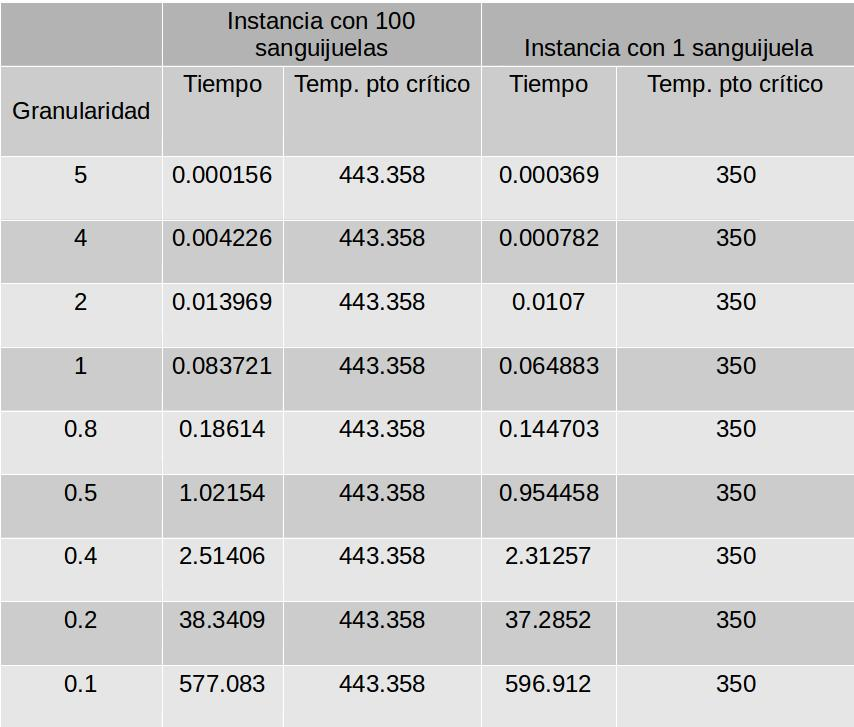
\includegraphics[scale=0.4]{instancias40x40_2.jpg}\caption{Para hacer esta última medición, decidimos dejar intacta la instancia con 100 sanguijuelas y modificar la instancia que tiene solo una sanguijuela. La modificación que efectuamos fue aumentar considerablemente el radio de la sanguijuela a un valor de 40, siendo antes 0.002. Podemos observar que los tiempos son significativamente menores, parecidos a los que tomamos al trabajar con la instancia de 100 sanguijuelas e incluso en algunos casos menores. Es importante observar también, que la temperatura en el punto crítico ahora es siempre la misma (350) y antes (cuando el radio era 0.002) variaba y a veces la sanguijuela era descartada (para las granularidades 4, 2, 0.8 y 0.4 de la tabla anterior).}
\end{figure}



\subsection{Experimento 3}


\subsubsection{Experimento para Hipótesis 1}
Se modelaron 3 instancias, todas con los mismos valores de altura, ancho, granularidad, y cantidad de sanguijuelas. Lo único que se modifico en cada instancia fue el radio de estas últimas, principalmente con la idea de que:
 \begin{itemize}
    \item 1° Instancia = Todas sanguijuelas unitarias.
    \item 2° Instancia = Mitad sanguijuelas unitarias, mitad no unitarias.
    \item 3° Instancia  = Todas sanguijuelas no unitarias.
 \end{itemize}
 La temperatura de las sanguijuelas no es relevante al experimento, ya que no nos agrega nada saber la temperatura del punto crítico al mismo, y por simplicidad las mismas fueron ubicadas en posiciones múltiplos de la granularidad \\


Los resultados obtenidos fueron los siguientes:

\begin{figure}[H]
    \centering
    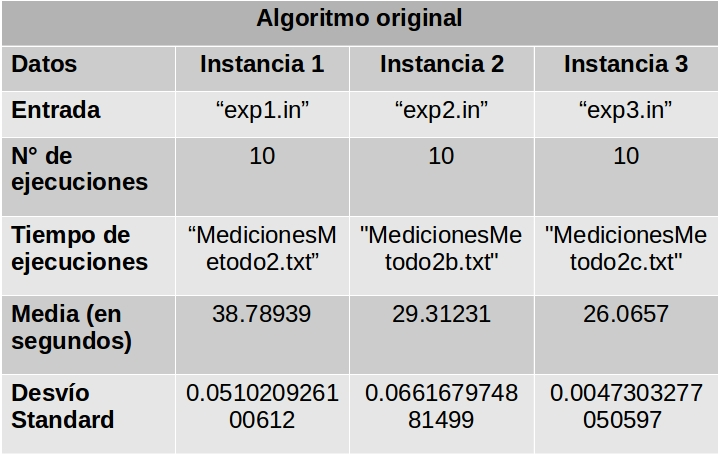
\includegraphics[scale=0.6]{graphs/tablaOriginal.jpg}
    \end{figure}
        
        
    \begin{figure}[H]
    \centering
    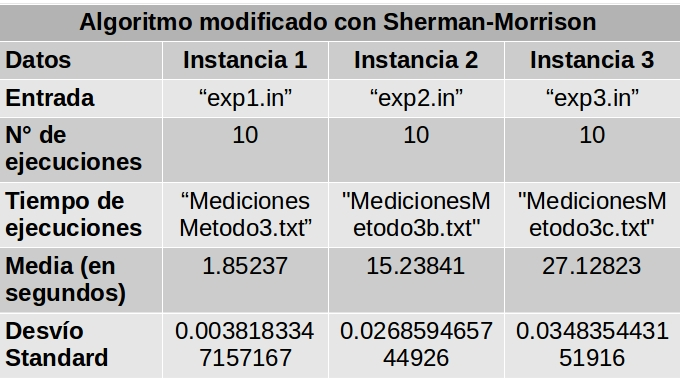
\includegraphics[scale=0.6]{graphs/tablaSherman.jpg}
    \end{figure}
        
        
 (Los archivos de entrada y los tiempos de corridas se puede encontrar en Experimentos/Experimento3).


    \begin{figure}[H]
    \centering
    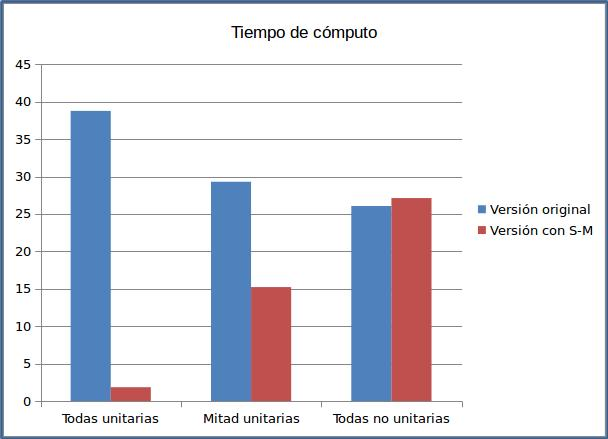
\includegraphics[scale=0.6]{graphs/graficoExp1.jpg}\caption{Gráfico obtenido de los valores de la media del tiempo de cada ejecución}
    \end{figure}
    
    
    
\subsubsection{Experimento para Hipótesis 2}
    Se modelaron 3 instancias, todas con los mismos valores de altura, ancho, cantidad de sanguijuelas, modificando la granularidad en cada una. El radio de las sanguijuelas se genero pseudoaleatoriamente con MATLAB en un rango posible de 0.1 a 16. Se eligió este rango para que el experimento sea más representativo con las granularidades elegidas para experimentar. Por simplicidad, las mismas fueron ubicadas en posiciones múltiplos de 16. Las instancias son las siguientes:
    
     \begin{itemize}
    \item 1° Instancia = Granularidad 8
    \item 2° Instancia = Granularidad 4
    \item 3° Instancia  = Granularidad 2
 \end{itemize}
 
  La temperatura de las sanguijuelas no es relevante al experimento, ya que no nos agrega nada saber la temperatura del punto crítico al mismo.
  
  Los resultados obtenido fueron los siguientes:
  
     \begin{figure}[H]
    \centering
    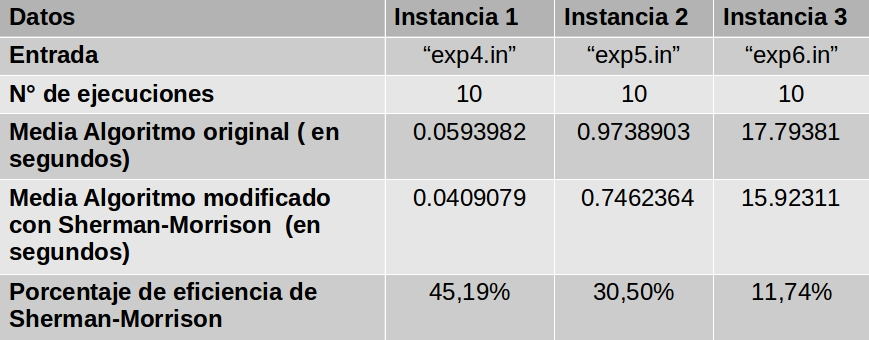
\includegraphics[scale=0.5]{graphs/grafico3.jpg}
    \end{figure}\
        
         (Los archivos de entrada y los tiempos de corridas se puede encontrar en Experimentos/Experimento3).


    \begin{figure}[H]
    \centering
    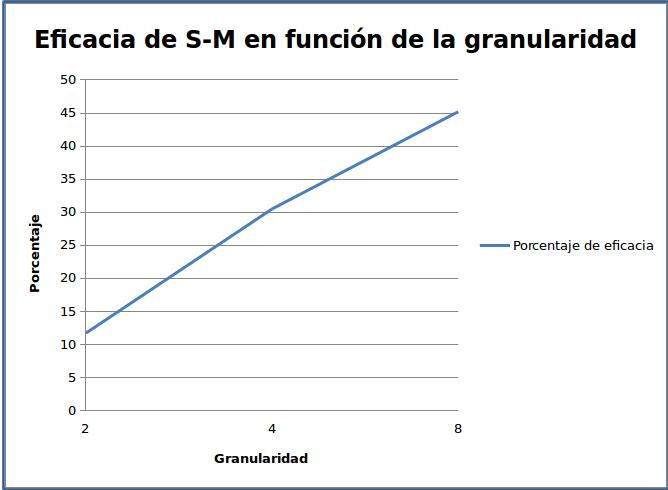
\includegraphics[scale=0.6]{graphs/graf.jpg}\caption{Gráfico obtenido de los valores del porcentaje de eficiencia del algoritmo con Sherman-Morrison comparándolo con el algoritmo original en función de la granularidad.}
    \end{figure}


